\documentclass{article}%
\usepackage[T1]{fontenc}%
\usepackage[utf8]{inputenc}%
\usepackage{lmodern}%
\usepackage{textcomp}%
\usepackage{lastpage}%
\usepackage[head=40pt,margin=0.5in,bottom=0.6in]{geometry}%
\usepackage{graphicx}%
%
\title{\textbf{Liberaron en Aragua a la activista política Rosa Virgina González}}%
\author{El Nacional Web}%
\date{13/11/2018}%
%
\begin{document}%
\normalsize%
\maketitle%
\textbf{URL: }%
http://www.el{-}nacional.com/noticias/politica/liberaron{-}aragua{-}activista{-}politica{-}rosa{-}virgina{-}gonzalez\_259566\newline%
%
\textbf{Periodico: }%
EN, %
ID: %
259566, %
Seccion: %
Política\newline%
%
\textbf{Palabras Claves: }%
Política, Presos políticos, Aragua\newline%
%
\textbf{Derecho: }%
1.2, %
Otros Derechos: %
1.10, 5, %
Sub Derechos: %
1.2.2, 1.10.1\newline%
%
\textbf{EP: }%
NO\newline%
\newline%
%
\textbf{\textit{Su detención había sido denunciada por Melva Paredes, diputada a la Asamblea Nacional~}}%
\newline%
\newline%
%
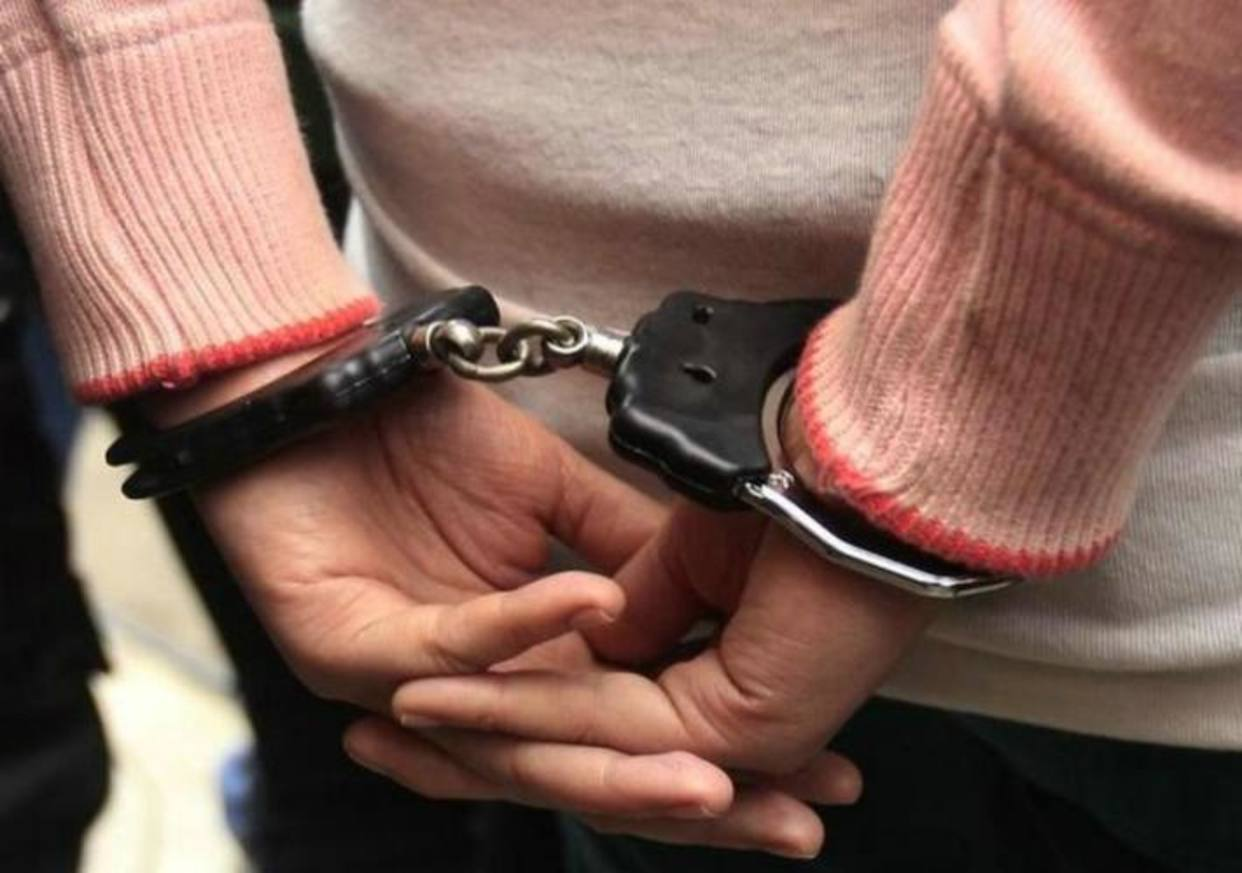
\includegraphics[width=300px]{190.jpg}%
\newline%
%
La activista política y estudiante Rosa Virginia González, fue liberada este martes luego de permanecer detenida desde el 13 de enero de 2018.%
\newline%
%
El Foro Penal Venezolano informó que la mujer fue absuelta de los cargos que tenía. Había sido privada de libertad por funcionarios del Servicio Bolivariano de Inteligencia Nacional (Sebin) en el estado Aragua.%
\newline%
%
Una periodista de Aragua informó que González era acusada de porte ilícito de arma de guerra y posesión de municiones.%
\newline%
%
Al momento de su detención a principios de año se desconocía el paradero de la activista, situación que fue denunciada por la diputada a la Asamblea Nacional (AN), Melva Paredes.%
\newline%
%
\end{document}